\documentclass{article}

\usepackage{verbatim}
\usepackage{color}
\usepackage[margin=1.2in]{geometry}
\usepackage{mathtools}
\usepackage{xcolor}
\usepackage{multirow}
\usepackage{caption}
\usepackage{subcaption}
\usepackage[allcolors=blue]{hyperref}
\hypersetup{
    colorlinks=true,
    linkcolor=blue,
    filecolor=magenta,      
    urlcolor=cyan,
}
\usepackage{pdfpages}
\usepackage[section]{placeins}
\usepackage{graphicx}

\usepackage{amsmath}
 \usepackage{amssymb}
 \usepackage{bm}
 
\DeclarePairedDelimiter\ceil{\lceil}{\rceil}
\DeclarePairedDelimiter\floor{\lfloor}{\rfloor}
\newcommand{\wid}{15cm}
\newcommand{\widsmall}{10cm}

\graphicspath{{../imgs/}}
 
\title{Hierarchical Variational Inference for Federated Learning.\vspace{1cm}}

\author{%
	\begin{tabular}{p{2cm} p{6.1cm} p{2cm} r}
		Student: & Anton Maksimov & Start Date: & 20 Mar 2020 \tabularnewline
		Advisors: & Luca Corinzia & End Date: &09 Oct 2020
	\end{tabular}
}

\date{}

\begin{document}

\includepdf[pages=-]{declaration-originality_signed.pdf}
\maketitle

\section*{Description}

Federated learning is a recently emerged paradigm describing learning of a model using a server and a network of devices. These devices, called clients, retain a private dataset and transmit and receive information to/from the server in the form of agglomerated updates. This setting has some advantages with respect to train many models separately and on training a single model on pooled data, such as delegation of computations from server to devices, increasing of the effective amount of training data and possibilities to perform learning in a more  secure and personalized way. These features solves many of the typical constraints found in applications, e.g.  limited and heterogeneous storage and computational power of the devices, and impossibility of pooling the datasets in a centralized settings due to limited bandwidth and privacy concerns.

One of the recent approaches in federated learning is the use of the variational inference to handle a multi-task learning setting. It was shown to tackle non-IID data and perform multi-task learning of non-convex models successfully competing with the current state-of-the-art methods. However, to the best of our knowledge variational federated learning has been applied only to mean-field models. The goal of the project is to extend this approach to the hierarchical models by using shared hyper-priors on the parameters of the client models and thus inducing new dependencies between them. Hierarchical models can be especially useful when the data inherently comes from several distinct clusters of sources, e.g. language models with different local variations.


\section*{Related Work}
The first known Federated Learning algorithm is \textit{FedAvg}~ \cite{FedAvg}. According to it a server performs averaging of client models, which are locally updated using stochastic gradient descent on private data. However, it was shown already in the original paper that FedAvg is not robust in case of non IID-data. One way to overcome this is to introduce proximal term which pushes local models not to deviate too much during one local updating round~ \cite{li2018federated}, though this modification still doesn't lead to consistently better than FedAvg learning over non--IID data~\cite{li2018federated}.

\textit{Multi-task learning (MTL)} aims at tackling this problem, having as a goal learning models for multiple related tasks simultaneously. It can be classified depending on how relationships between tasks are introduced: if their structure is known \textit{a priori} or it should be inferenced from the data~\cite{smith2017federated} (hard and soft parameter sharing correspondingly), if we would like to improve the performance of all the tasks simultaneously or only for some subset of them (symmetric and asymmetric MTL)~\cite{Zhang2010}.

Distributed MTL aims at learning from data distributed over a network. In a federated setting the structure between models fitted to local datasets frequently exists and this fact makes it possible to improve the learning~\cite{smith2017federated, Goncalves}. Nevertheless, the approach proposed in \cite{smith2017federated} allows to handle only convex losses, which are not applicable to deep learning models. In order to overpass this limitation one can use \textit{variational inference}~\cite{corinzia2019variational}. This technique makes it possible to efficiently learn over highly non--IID data distributions.

One of the improvements of this method could be the expanding the star--shaped Bayesian network of parameters to a hierarchical one \cite{ranganath2015hierarchical}, where distributions of the modes parameters are defined by the other hyper-priors distribution which are learned during the optimization. The learning method should allow flexible generalization of common network knowledge and specialization of nodes according to their local data \cite{nguyen2020distributed}. Different variational inference methods, such as black-box variational inference \cite{ranganath2013black} or normalizing flows \cite{rezende2015variational} could be used.

Note, that the notion of \textit{hierarchical federated learning} can be used in a sense of introducing additional layer of auxiliary servers which first collect data from their children clients in order to reduce communication cost (e. g. structure server~---~cell base stations~---~connected to them mobile users \cite{Liu2019, Abad2020}), but this type of hierarchy differs from considered in this work, as it assumes that all clients have common data generating process and hierarchy comes from the construction of the communication network, whereas we consider clients belong to several different groups with their own data generating processes, which means hierarchy of their latent parameters.

 \begin{center}
 \captionof{table}{Initial plan}
 {\def\arraystretch{1.2}\tabcolsep=10pt
 
	\begin{tabular}{c p{15cm}}
		\hline
		Nr. & Work Package \\
		\hline
		1 & Review literature  \\
		2 & Implement hierarchical Bayesian network on the MNIST data splitted according to digits similarity \\
        3 & Extend approach to other FL datasets (FEMNIST, VSN, HAR, Shakespeare etc.) \\
        4 & Implement variation of Virtual algorithm with additional shared hyper-prior on simple datasets \\
        5 & Outline of written thesis  \\
		6 & Draft of written report  \\
		7 & Hand-In written report \\
		\hline
	\end{tabular}
}
\end{center}
\section*{Theory derivation for hierarchical federated update}
Having $K$ clients, $\theta$ are server parameters (network weights $(\boldsymbol{\mu}^s, \boldsymbol{\sigma}^s)$, $\phi_i$ are the corresponding client parameters $(\boldsymbol{\mu}_i^c, \boldsymbol{\sigma}_i^c)$, and corresponding to server and clients $\lambda_i^s$ and $\lambda_i^c$ (s. t. $\lambda^s= \{\lambda_i^s\}_{i=1}^K, \lambda^c= \{\lambda_i^c\}_{i=1}^K$) are the group assignment distributions with $G$ groups (simplexes in $\mathbb{R}^G$, which we assume to have uniform prior distributions there).

We have a mean--field proxy posterior distribution:
$$q(\theta, \phi, \lambda )=s(\theta, \lambda^{s}) \: c(\phi, \lambda^{c})
=\left(\prod_{i=1}^{K} s_i\left(\theta, \lambda^{s}\right)\right)
\left(\prod_{i=1}^{K} c_{i}\left(\phi_{i}, \lambda_{i}^{c}\right)\right)$$
where we are considering every distribution to be a Gaussian mixture of $G$ groups
\begin{equation*}
  \begin{cases}
s_{i}\left(\boldsymbol{\theta}, \lambda_{i}^{s}\right)
= \sum_{j=1}^G \lambda_i^s(j) \:\mathcal{N}\left(\boldsymbol{\mu}^s(j), \boldsymbol{\sigma}^s(j)\right)\\
c_{i}\left(\phi_{i}, \lambda_{i}^{c}\right)
= \sum_{j=1}^G \lambda_i^c(j)\:\mathcal{N}\left(\boldsymbol{\mu}^c(j), \boldsymbol{\sigma}^c(j)\right)
\end{cases}  
\end{equation*}


Following the idea of \cite{corinzia2019variational}, we then rewrite KL--divergence and get updating rule for weights
$$\begin{array}{c}
D_{KL}\left(s^{(t)}(\boldsymbol{\theta}, \lambda^s)\:c^{(t)}(\phi,  \lambda^c)
\bigg\vert\bigg\vert\frac{s^{(t)}(\theta, \lambda^s)\:c^{(t)}(\phi,  \lambda^c)}{s_i(\theta, \lambda^s)\:c_i(\phi_i,  \lambda_i^c)}\:p(\theta, \phi_i, \lambda^s, \lambda_i^c|\mathcal{D}_i)\right)\\

=\int d \boldsymbol{\lambda}^s \int d \boldsymbol{\theta}\: s^{(t)}(\boldsymbol{\theta}, \lambda^s)\: \log s_{i}(\boldsymbol{\theta}, \lambda_i^s)\: \underbrace{\int d \boldsymbol{\phi}\: d\boldsymbol{\lambda}^c\: c^{(t)}(\boldsymbol{\phi}, \lambda^c)}_{=1}
\newline 
+\int d \boldsymbol{\phi}\:d \boldsymbol{\lambda^c}\: c^{(t)}(\boldsymbol{\phi}, \lambda^c) \log c_{i}\left(\boldsymbol{\phi}_{i}, \lambda_i^c\right) \underbrace{\int d\boldsymbol{\theta}\:d \boldsymbol{\lambda^s}\: s^{(t)}(\boldsymbol{\theta}, \lambda^s)}_{=1}\:  -\\

\qquad-\bigg\int d \boldsymbol{\lambda^s}\int d \boldsymbol{\lambda^c}\int d \boldsymbol{\theta}\int d \boldsymbol{\phi}\: s^{(t)}(\boldsymbol{\theta}, \lambda^s)\: c^{(t)}(\boldsymbol{\phi}, \lambda^c) \log p\left(\boldsymbol{\theta}, \boldsymbol{\phi}_{i}, \lambda^s, \lambda_i^c\mid \mathcal{D}_{i}\right)\\

=\int d \boldsymbol{\lambda}^s 
\int d \boldsymbol{\theta}\: \underbrace{s^{(t)}(\boldsymbol{\theta}, \lambda^s)}_{s_{i}(\boldsymbol{\theta}, \lambda_i^s)\frac{ s^{(t-1)}(\boldsymbol{\theta}, \lambda^s)}{s_i^{(t-1)}(\boldsymbol{\theta}, \lambda_i^s)}}
\log \frac{s_{i}(\boldsymbol{\theta}, \lambda_i^s)\: s^{(t)}(\boldsymbol{\theta}, \lambda^s)}{s^{(t)}(\boldsymbol{\theta}, \lambda^s)\: p(\boldsymbol{\theta})}

+\int d \boldsymbol{\lambda}_i^c \int d \boldsymbol{\phi}_{i} c_{i}^{(t)}\left(\boldsymbol{\phi}_{i}, \lambda_i^c\right) \log \frac{c_{i}^{(t)}\left(\boldsymbol{\phi}_{i},  \lambda_i^c\right)}{p\left(\boldsymbol{\phi}_{i}\right)} - \\

\qquad-\int d \boldsymbol{\lambda}^s\int d \boldsymbol{\lambda}_i^c\int d \boldsymbol{\theta}\: s^{(t)}(\boldsymbol{\theta}, \lambda^s) \int d \boldsymbol{\phi}_{i}\: c_{i}^{(t)}\left(\boldsymbol{\phi}_{i}, \lambda_i^c\right) \left(\log p\left(\mathcal{D}_{i} \mid \boldsymbol{\theta}, \boldsymbol{\phi}_{i}, \lambda^s, \lambda_i^c\right) - \underbrace{\log p\left(\mathcal{D}_{i}\right)}_{\text{const}} 
- \underbrace{\log \frac{1}{p(\lambda^s)}}_{\text{const}} - \underbrace{\log \frac{1}{p(\lambda_i^c)}}_{\text{const}}\right)
\end{array}$$
using normalisation of pdfs and Bayesian rule $p\left(\boldsymbol{\theta}, \boldsymbol{\phi}_{i}, \lambda^s, \lambda_i^c\mid \mathcal{D}_{i}\right)
=
\frac{p\left(\mathcal{D}_{i} \mid \boldsymbol{\theta}, \boldsymbol{\phi}_{i}, \lambda^s, \lambda_i^c\right) p(\boldsymbol{\theta}) p(\boldsymbol{\phi}_{i}) p(\lambda^s) p(\lambda_i^c)}{p(\mathcal{D}_i)}. 
$ Constants in the end (because of initial uniform priors) lead to the constant shift of the loss, therefore not influencing the result, and could be dropped.
Therefore, using the fact that $\dfrac{s_{i}(\boldsymbol{\theta}, \lambda_i^s)}{ s^{(t)}(\boldsymbol{\theta}, \lambda^s)} 
= \dfrac{s_{i}^{(t-1)}(\boldsymbol{\theta}, \lambda_i^s)}{ s^{(t-1)}(\boldsymbol{\theta}, \lambda^s)}$ we obtain the loss of update
$$\begin{array}{c}
\mathcal{L}(s_i(\boldsymbol{\theta}, \lambda^s), c_i(\boldsymbol{\phi}_{i}, \lambda^s) = D_{KL}\left(s_{i}(\boldsymbol{\theta}, \lambda_i^s)\frac{ s^{(t-1)}(\boldsymbol{\theta}, \lambda^s)}{s_i^{(t-1)}(\boldsymbol{\theta}, \lambda_i^s)}\bigg\vert\bigg\vert p(\boldsymbol{\theta})\frac{ s^{(t-1)}(\boldsymbol{\theta}, \lambda^s)}{s_i^{(t-1)}(\boldsymbol{\theta}, \lambda_i^s)}\right) 
+ D_{KL}\left(c_{i}^{(t)}\left(\boldsymbol{\phi}_{i}, \lambda_i^c\right) \big\vert\big\vert p\left(\boldsymbol{\phi}_{i}\right)\right) \: 
-\\ \vspace{0.5cm}
\qquad \mathbb{E}_{\substack{s^{(t)}(\boldsymbol{\theta}, \lambda^s)\\
c_{i}^{(t)}\left(\boldsymbol{\phi}_{i}, \lambda_i^c\right)}} \log p\left(\mathcal{D}_{i} \mid \boldsymbol{\theta}, \boldsymbol{\phi}_{i}, \lambda^s, \lambda_i^c\right)

\end{array}$$
which is very similar to the non-hierarchical one in~\cite{corinzia2019variational}.

\section*{Practical part}
\subsection*{Model description}


First, we implement the non-federated hierarchical Bayesian neural network following the paper on gesture classification~\cite{Gestures}, for which we were not able to find the code. For the structure description see the fig.~\ref{structure}.

We don't use layers of \textit{tensorflow-probability} and produce code almost from scratch being inspired by the code from the Krasser's blog~\cite{krasser_blog} as an illustration to the paper~\cite{blundell2015weight}, using \textit{TensorFlow Functional API}. We adapt it to the MNIST dataset with several groups represented by handwritten digits which are somehow similar from human (ours) point of view (e.g. 1 is similar to 7, 2 -- to 5 etc. We use 3 such a groups). For the TensorFlow model structure see the fig.~\ref{tf_structure}.

The loss consists of estimated by sampling ELBO and added to it cross-entropy between the layer output and the true label. Overall weight of ELBO is the same as the cross-entropy loss and is scaled accordingly to the number of groups in the hierarchy.

\begin{figure}[h!]
	\centering
	\begin{minipage}{17cm}
		\subfloat[][Weights sets ("zero" and "group-wise") and datasets of the network]{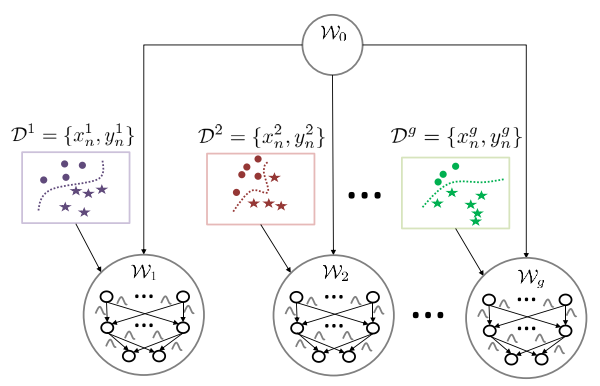
\includegraphics[width=9cm]{hierarchical.png}}
        \hfill
        \vspace{0.2cm}
		\subfloat[Graphical representation of the model. Group-wise weights (their mean and variance as assumed normal distributions) $\mathcal{W}_g$ have learnable prior $\tau_g$ relative to "zero"-weights $\mathcal{W}_0$. They have their own "wide" priors $v$ and $\tau_0$. Group membership $z_n$ (exactly known or deduced) affects the final class $y_n$, which is found using it, the feature $x_n$ and~$\mathcal{W}_g$.  ]{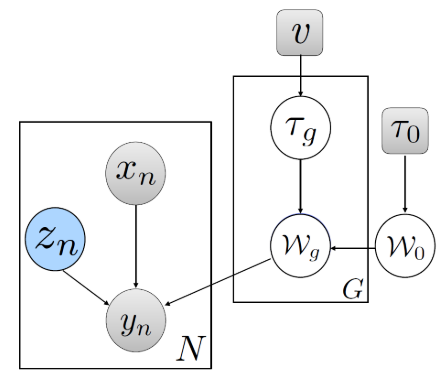
\includegraphics[width=7.5cm]{model.png}}
		
		\caption{Structure of the hierarchical Bayesian non-federated model, pictures are taken  from~\cite{Gestures}.}
			\label{structure}
	\end{minipage}

\end{figure}

\begin{figure}[h!]
	\centering
		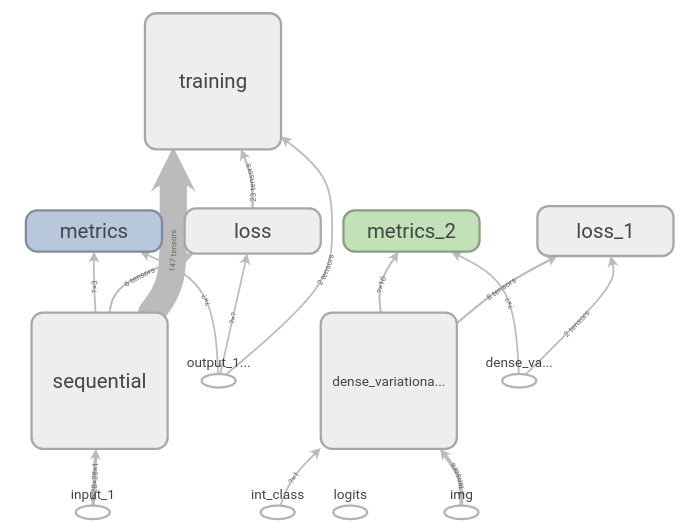
\includegraphics[width=14cm]{graph.png}
	\caption{Full model structure. The left part (LeNet~\cite{lenet} structure) predicts probabilities of group-membership (we used 3 groups), then its output is used in the right part (dense variational grouped layer) in "predicting" mode, where it uses logits from the left part instead of integer exact memberships, whereas exact ones are used in the model's "training" mode.}
	\label{tf_structure}
\end{figure}

\subsection*{Experiments}
The code is available on \href{https://github.com/antmaxi/Hierarchical-Variational-Learning}{github}.
Data from MNIST is shuffled and divided as 60000 digits for training and 10000 for testing.

As the main class-inference model we use single dense variational layer with no activation (surprisingly, Softmax or ReLU activation don't allow to train the model effectively, as, probably, the output during training is, according to~\cite{Gestures}, the weighted sum of group-wise calls on the data, and non-linear activation somehow destroys this additive nature of the model).

For Monte-Carlo sampling in order to estimate the resulting class membership probabilities we use only 5 samples, as with bigger amount, as we noticed, initial learning is more spurious, see fig.~\ref{sampling} (because probably increased amount of samples which are too far from the mean makes the loss blow-up at some steps).%(slow probably because there is not enough asymmetry for training of initially symmetric weights; might be useful in future to increase number of sampling as the learning progresses and the more subtle properties of distribution need to be found).

The "group-inference" LeNet model is trained for 100 epochs till saturation.

Other the best used parameters: $\tau_0^{-1} = 1, v = 0.3, \text{learning rate}=0.1$, the same parameters are near-the-best for non-hierarchical training (except $v$, which it doesn't have).
\subsection*{Results}
Resulting test accuracy after 100 epochs much bigger~(table \ref{table_res}) than the one of the model with non-hierarchical variational inference (VI) with the best found prior scale. It is also better than when using simple dense layer. 

For dynamics of accuracy on train and test data for hierarchical and non-hierarchical variational models, see fig.~\ref{acc}

\begin{figure}
	\centering
	\begin{minipage}{17.5cm}
		\subfloat[Test accuracy]{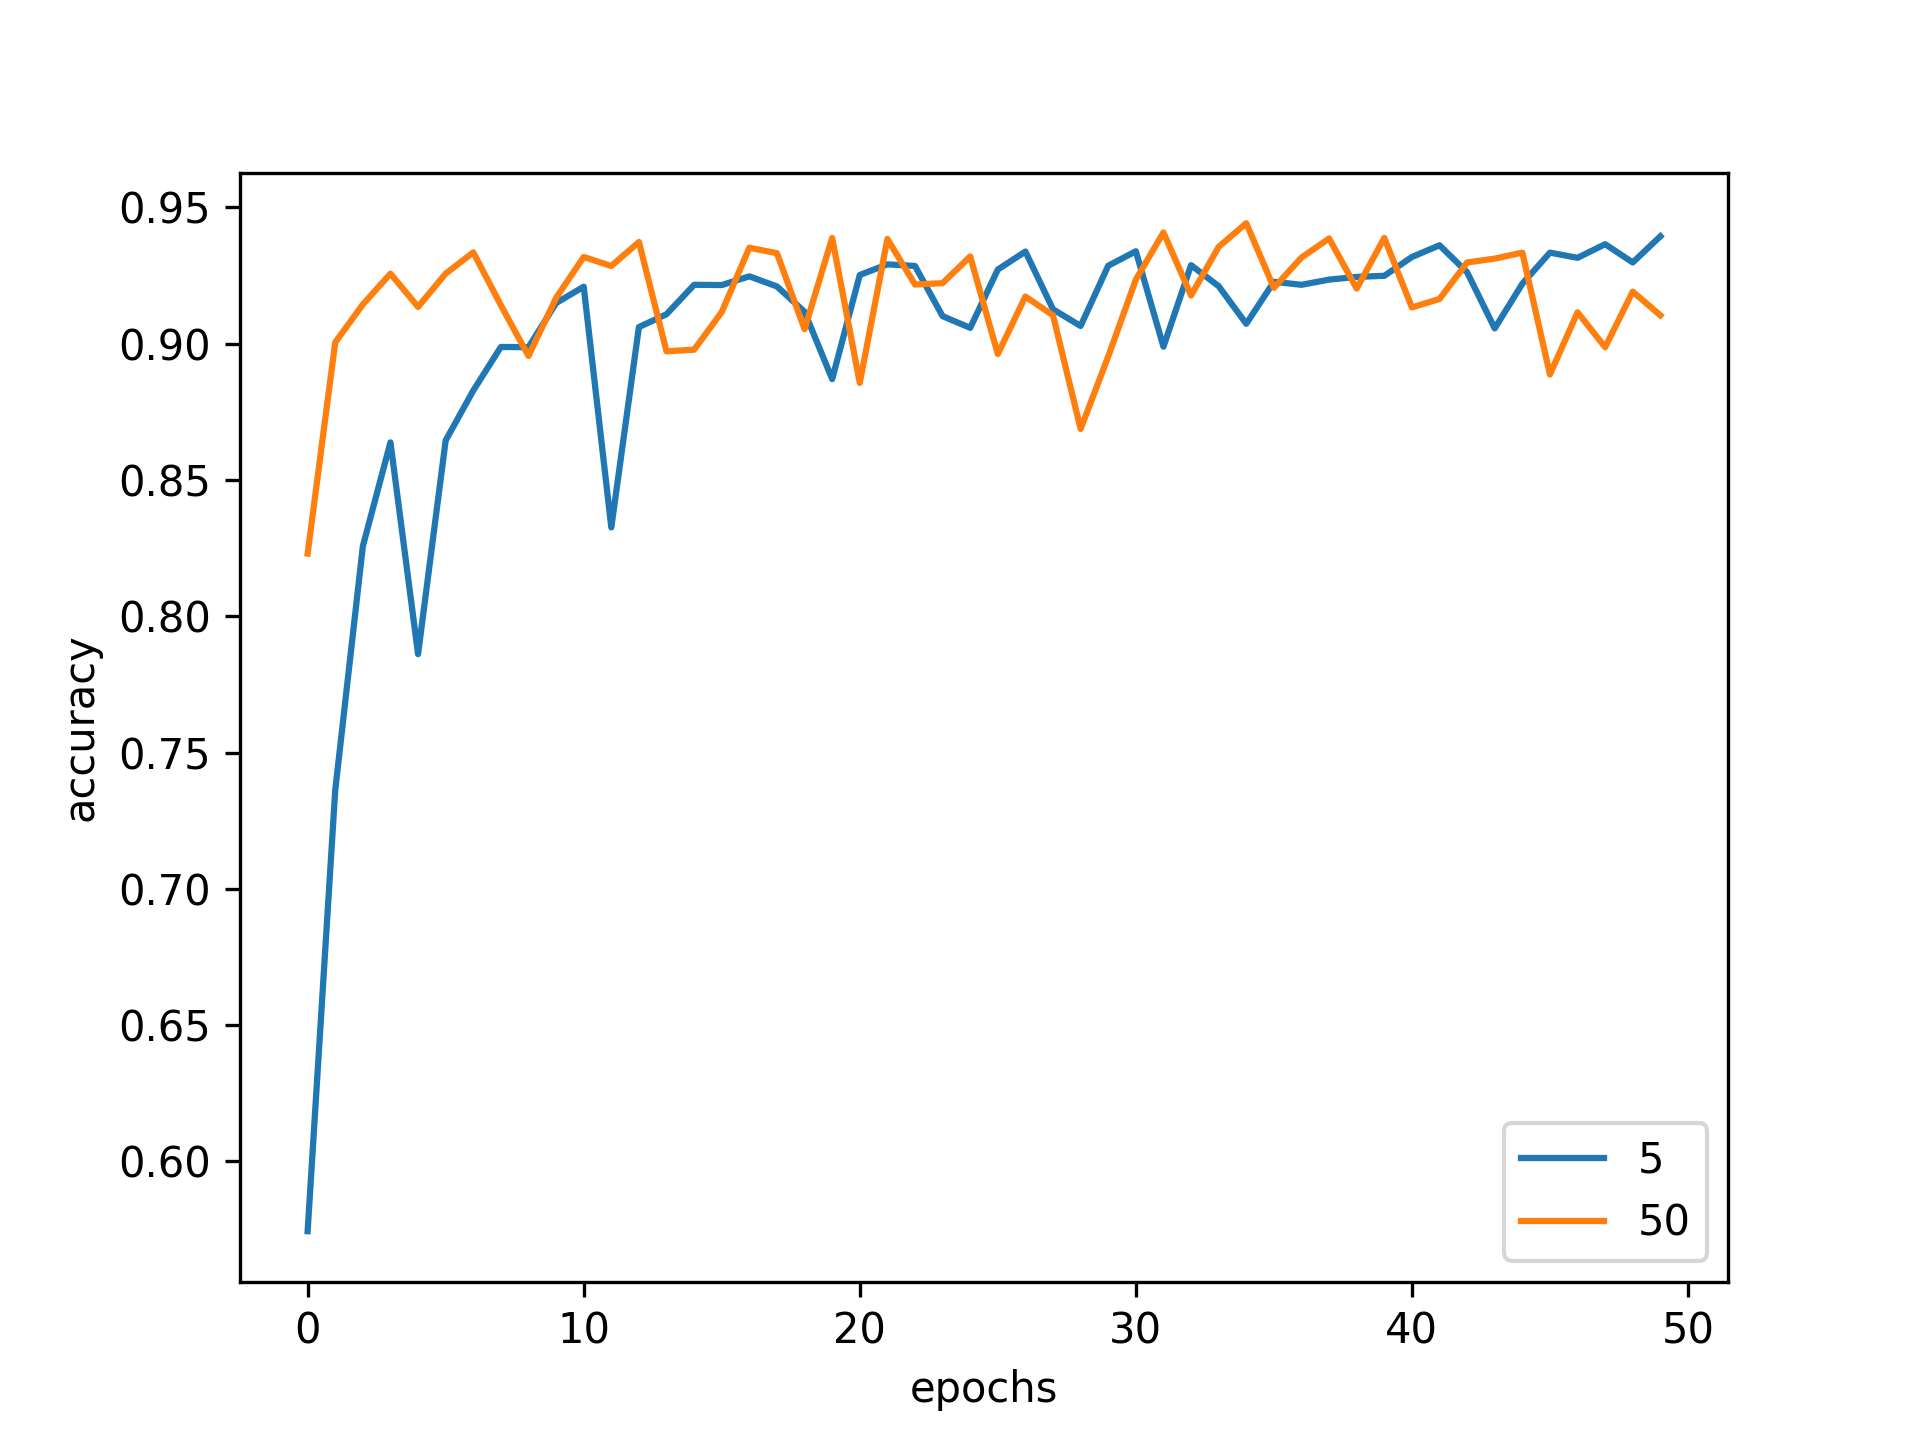
\includegraphics[width=8.5cm]{accuracy_sample.png}}
        \hfill
        \vspace{0.0cm}
		\subfloat[Test loss  ]{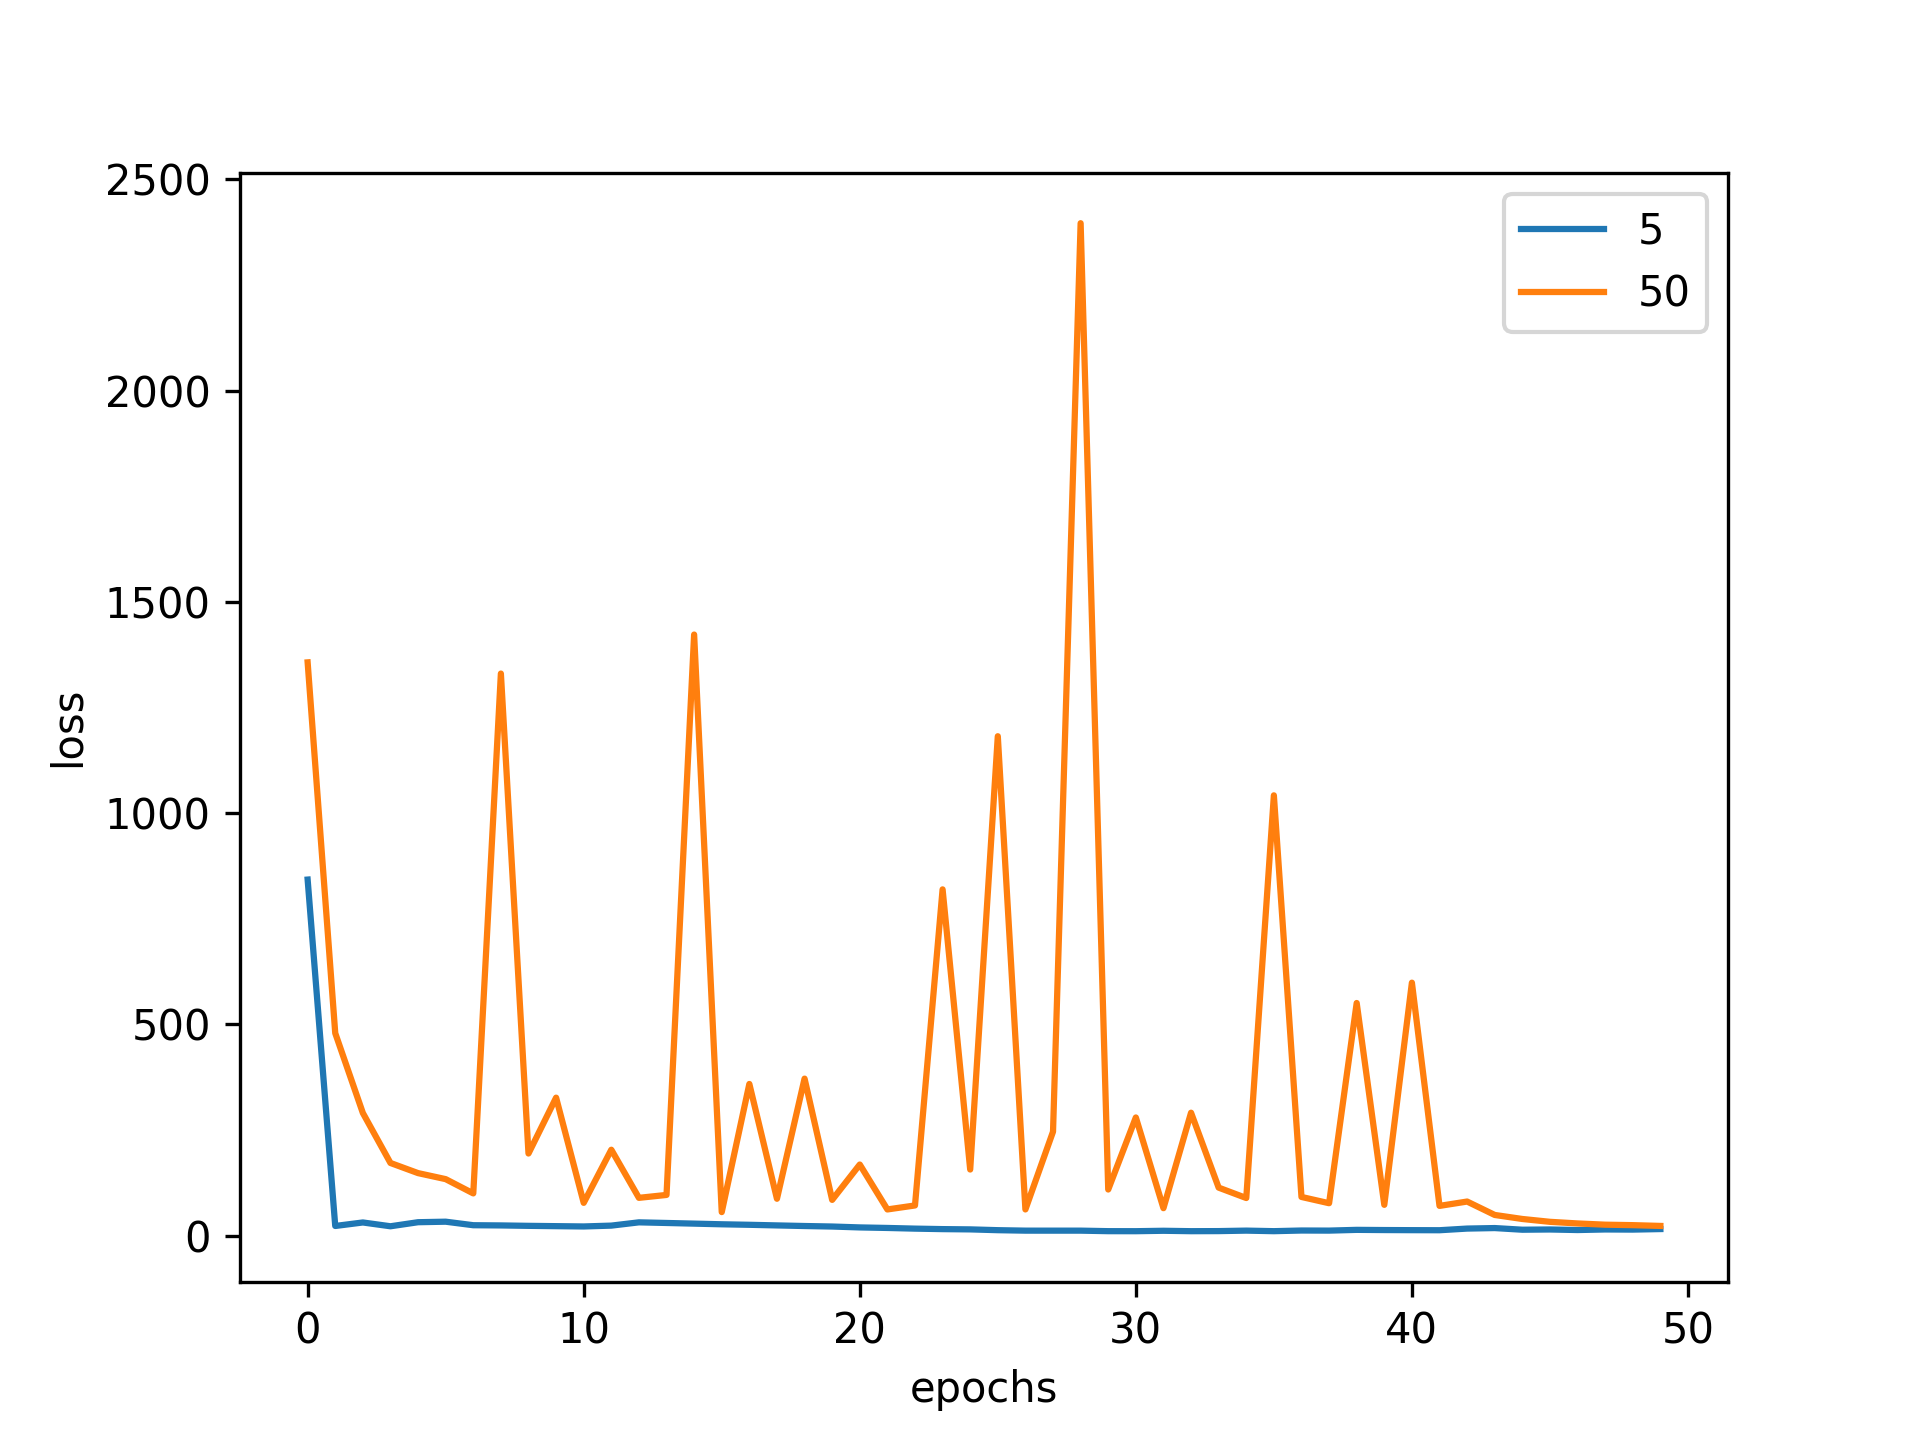
\includegraphics[width=8.5cm]{loss_sample.png}}
		
		\caption{Difference when changing sampling number in hierarchical model.}
			\label{sampling}
	\end{minipage}
\end{figure}	

\begin{figure}
	\centering
		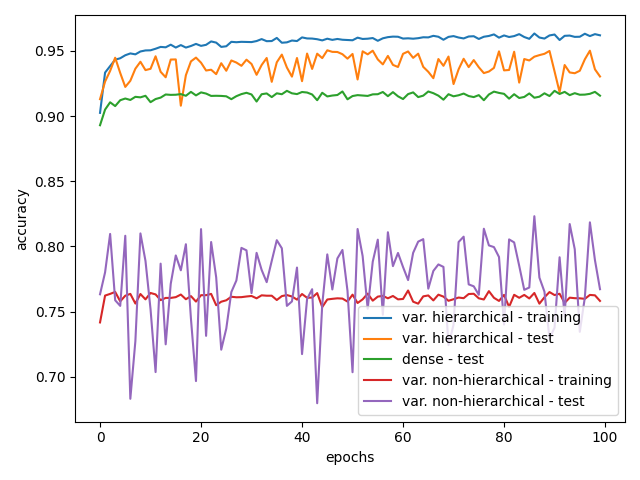
\includegraphics[width=\wid]{accuracy.png}
	\caption{Training and testing accuracy during training for different methods. Variational methods have bigger variance of result, which could potentially be tackled by reducing learning step and increasing sample number in late training stages, or implementing Local Reparameterization~\cite{localReparam} instead of usual non-centered reparameterization. Plus hierarchical method improves over non-hierarchical and has lesser variance too.}
	\label{acc}
\end{figure}	

To test whether the weights corresponding to the groups of digits really train specifically, we plot on the fig.~\ref{groups} the accuracy of prediction depending on the true label.

\begin{figure}
	\centering
		\caption{Accuracy of prediction depending on the true label for different types of weights and throughout training procedure.}
	\begin{minipage}{\wid}
		\subfloat[][1 epoch of training. Not yet specialized weights, especially "zero" ones.]{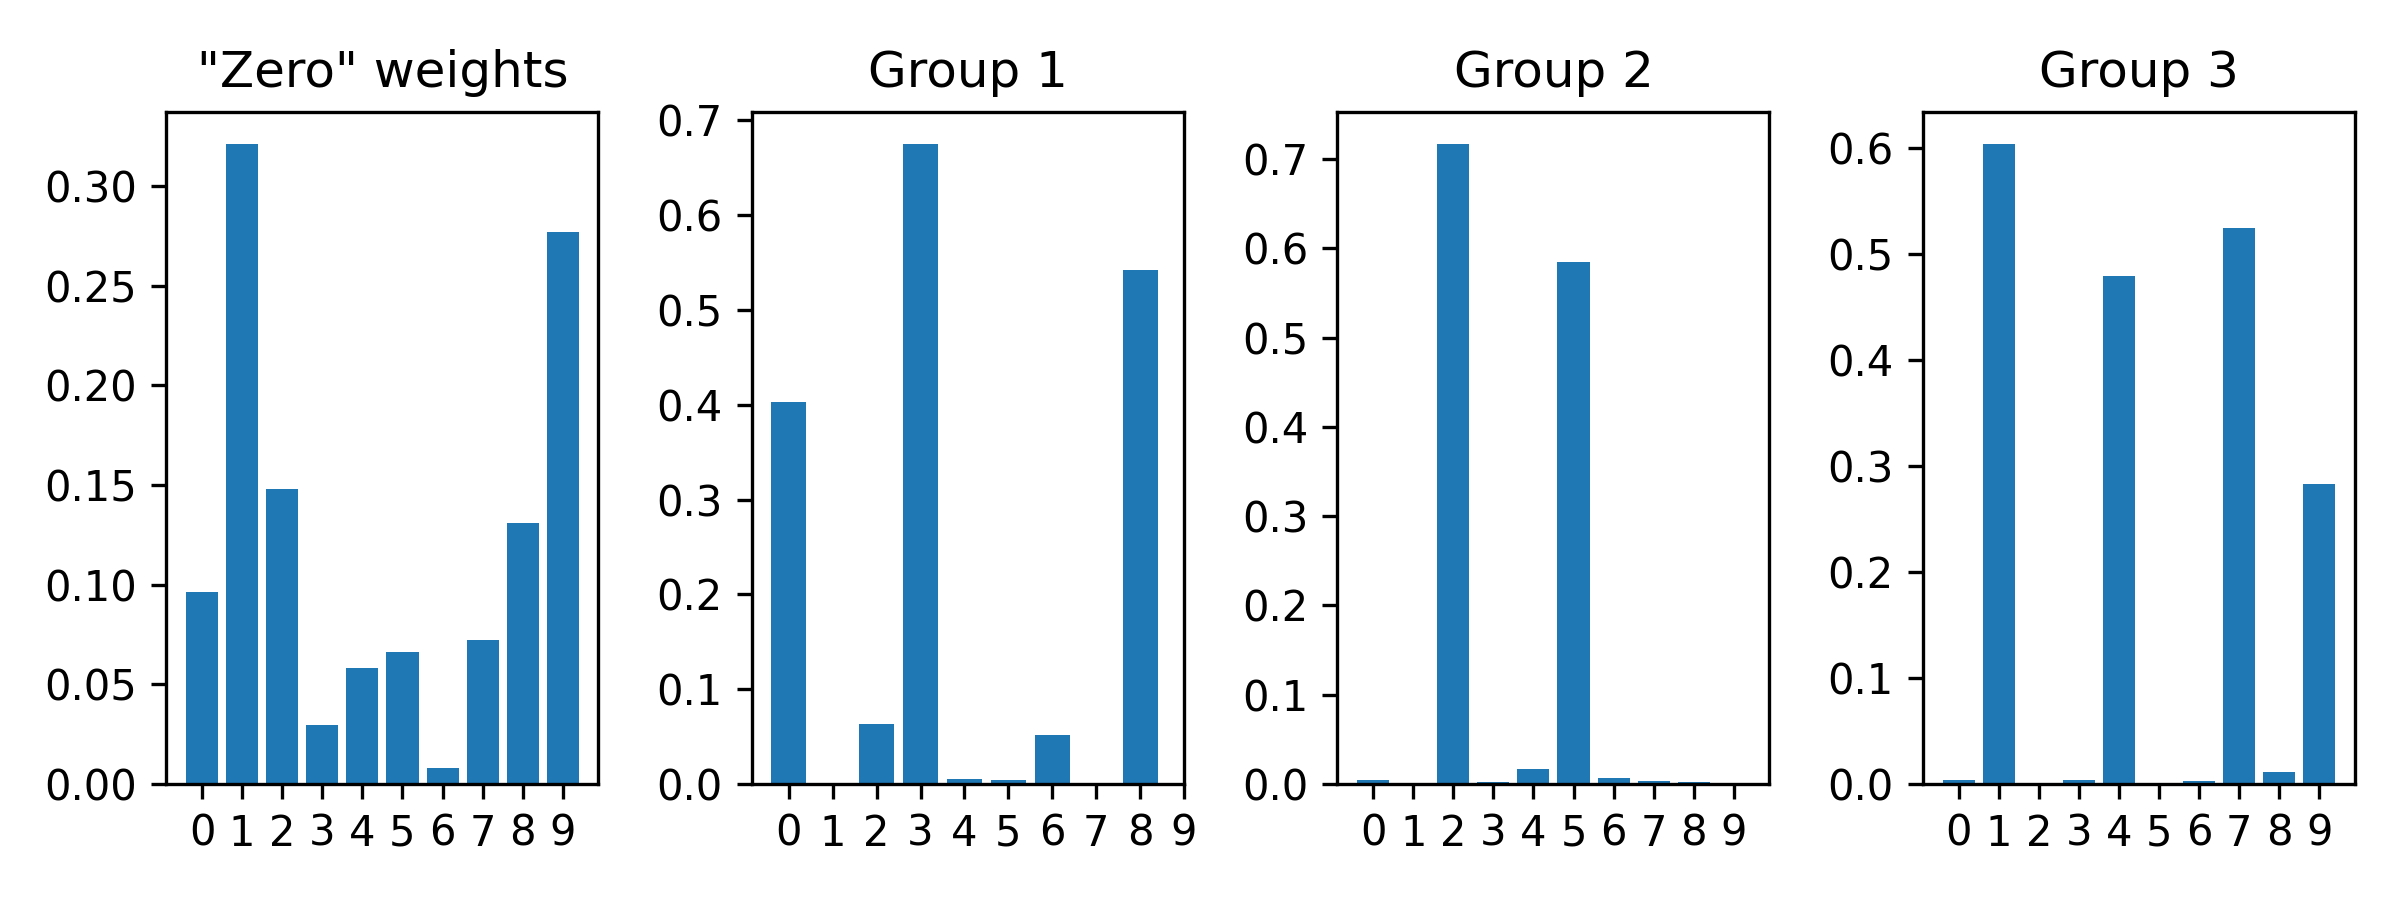
\includegraphics[width=\wid]{1-epochs.png}}
        
        \subfloat[10 epochs of training. almost specialize group-wise weights, "zero" ones are starting to drift to the 2nd group.]{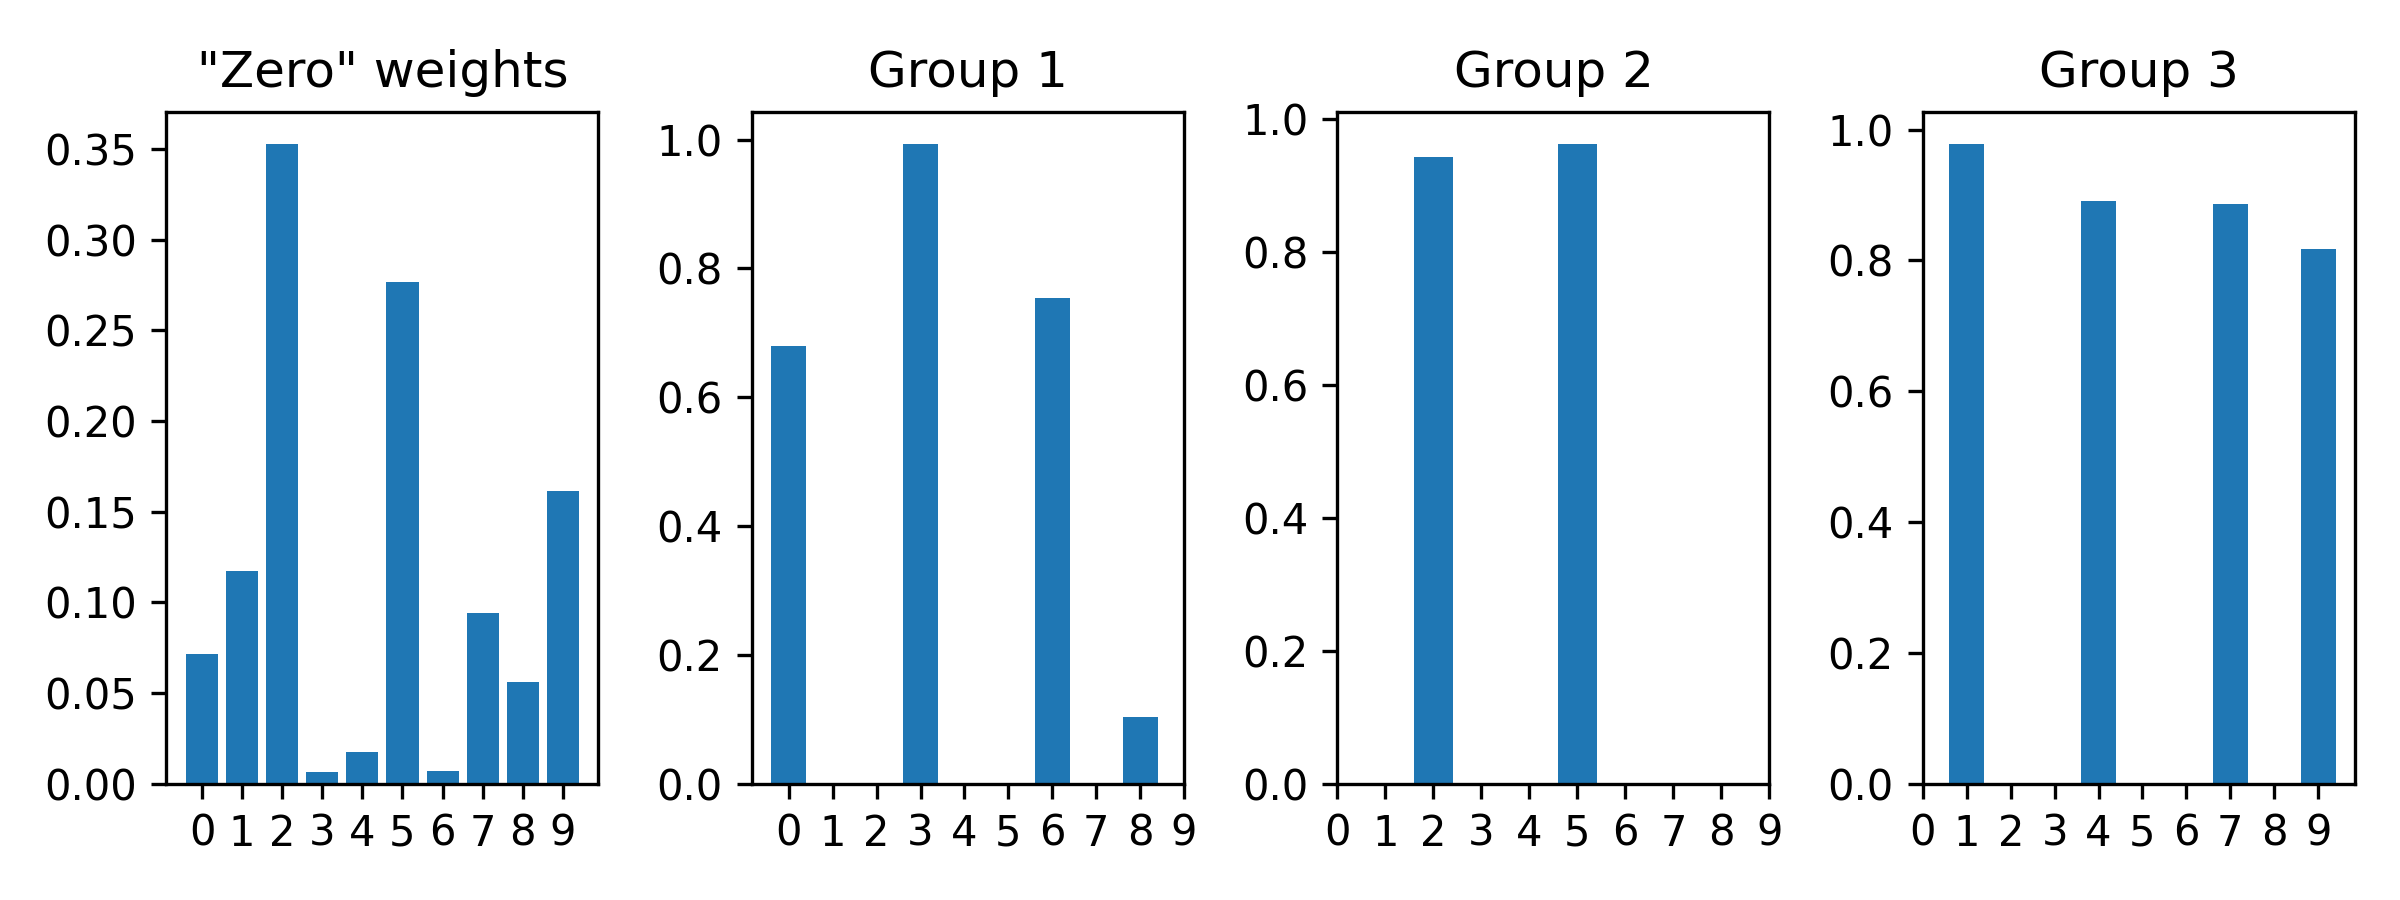
\includegraphics[width=\wid]{10-epochs.png}}
        
		\subfloat[100 epochs of training. Specialized group weights (according to our prior assignment), "zero" ones are close to one of the groups (2nd)]{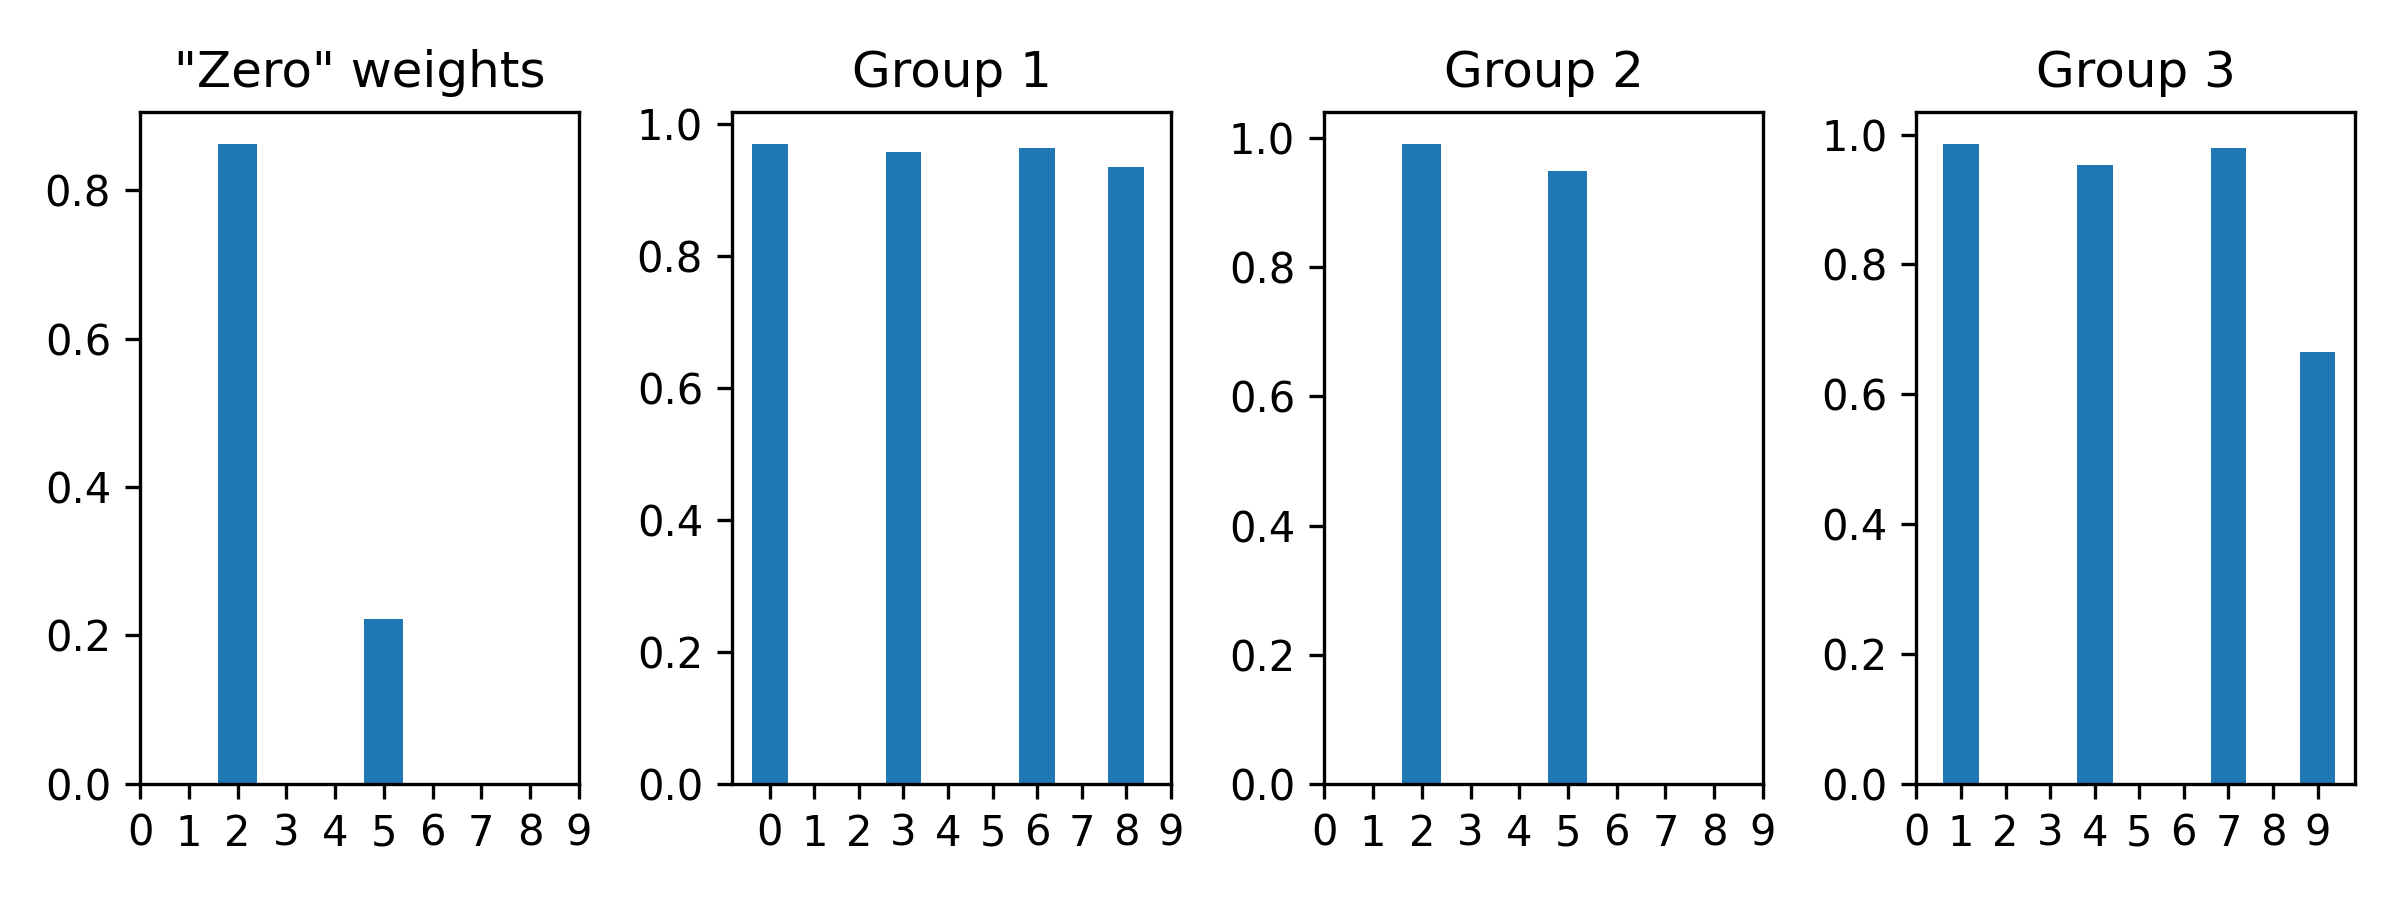
\includegraphics[width=\wid]{100-epochs.png}}
			\label{groups}
	\end{minipage}

\end{figure}

%\centering
\begin{table}[!]
	%\hspace{1.5cm}
	\centering
	\begin{tabular}{|l|c|}
		\hline
		Type & Test accuracy \\ \hline
		Dense - softmax & $0.916 \pm 0.003$ \\
		Variational non-hierarchical & $0.79 \pm 0.02$
		\\
		Variational hierarchical & $0.937 \pm 0.003$\\ \hline
	\end{tabular}
\caption {Comparison of methods' test accuracy after 100 epochs on single layer, each run is done for 5 repetitions with shuffled data}
\label{table_res}
\end{table}

\section*{Resume}
\begin{itemize}
    \item Hierarchical variational model improves in terms of accuracy over simple dense and non-hierarchical variational ones when tested on MNIST dataset.
    \item The variance of hierarchical model is also less than of non-hierarchical one. 
\end{itemize}
\section*{Future research}
\begin{itemize}
    \item Modification of the model for other types of data.
    \item Implementation of the federated type parameters' updates.
\end{itemize}
\newpage
%%%%%%%%%%%%%%%%%%%%%%%%%%%%%%%%%%%%%%%
 \section*{Project Specific Expectations}
These goals express the expectations w.r.t which the work will be evaluated. This list should provide a reference, but not a simple checklist - independent initiative by the student which leads to results not listed here is encouraged. 

\subsection*{Minimum Expectations}
Implementation of the hierarchical Bayesian neural network \cite{Gestures} and its testing.

\subsection*{Expectations}
Development of the algorithm for hierarchical variational federated learning using shared hyper-prior on the Virtual original algorithm. Its practical implementation and testing on real--world data. Several variational inference methods and datasets used.

\subsection*{Above Expectations}
Exploration of new ideas in the area of hierarchical latent variational model in the area of F-MTL.

\section*{General Expectations}
The following expectations are based on the evaluation sheet used for this thesis\footnote{\url{https://www.ethz.ch/content/dam/ethz/special-interest/itet/department/Studies/Forms/SAMA_Bewertungsblatt_EN.pdf}}. They should provide a general orientation about the expected workstyle and conduct.

\subsection*{Minimum Expectations}
The student acquires a solid working knowledge of the relevant concepts and is therefore able to participate in discussions and implement the thesis.
All work performed is well structured and documented as to enable efficient follow-up work. In addition to continuous documentation, this is particularly true for the final written thesis.
All tasks which are agreed upon by supervisor and student are implemented.
The expected quality of results  corresponds to what the student can possibly achieve in the absence of major unexpected problems.
The main contents of the thesis are presented in an informative but concise talk to an expert audience.

\subsection*{Expectations}
The student acquires a good working knowledge of the relevant concepts and is therefore able to contribute in discussions and efficiently implement the thesis.
Documentation of the performed work uses all good practice tools which are available for this purpose. The final report reflects the student's good knowledge about the relevant topics and enables detailed comprehension the thesis' contributions.
In addition to the agreed tasks, the student regularly extends his research to questions which arise naturally during the work, but have not been discussed explicitly.
The quality of the results corresponds to what is feasible in the context of a student thesis.
The final presentation includes careful processing and structuring of the contents in order to effectively and illustratively convey information to the audience.

\subsection*{Above Expectations}
The student independently acquires knowledge which enables new perspectives and provides innovative suggestions. Documentation follows standards without compromises and shows a high commitment to detail while being efficiently useable by others. This applies especially to the use for a potential publication.
There is a regular and significant attempt to explore all  implications of the discussed tasks and make extensions and beneficial modifications to the original questions.
The quality of the results is as good as the problem permits, major problems are solved if possible and indicate a high student performance.
The final presentation delivers an impressive account of the thesis. The preparation and structure enables a seamless information flow. Great care is recognizable in the illustrations and graphics. The audience is captured and challenged.

\bibliographystyle{ieeetr}
\bibliography{references}

\end{document}